\documentclass[twoside]{book}

% Packages required by doxygen
\usepackage{calc}
\usepackage{doxygen}
\usepackage{graphicx}
\usepackage[utf8]{inputenc}
\usepackage{makeidx}
\usepackage{multicol}
\usepackage{multirow}
\usepackage{fixltx2e}
\PassOptionsToPackage{warn}{textcomp}
\usepackage{textcomp}
\usepackage[nointegrals]{wasysym}
\usepackage[table]{xcolor}

% Font selection
\usepackage[T1]{fontenc}
\usepackage{mathptmx}
\usepackage[scaled=.90]{helvet}
\usepackage{courier}
\usepackage{amssymb}
\usepackage{sectsty}
\renewcommand{\familydefault}{\sfdefault}
\allsectionsfont{%
  \fontseries{bc}\selectfont%
  \color{darkgray}%
}
\renewcommand{\DoxyLabelFont}{%
  \fontseries{bc}\selectfont%
  \color{darkgray}%
}
\newcommand{\+}{\discretionary{\mbox{\scriptsize$\hookleftarrow$}}{}{}}

% Page & text layout
\usepackage{geometry}
\geometry{%
  a4paper,%
  top=2.5cm,%
  bottom=2.5cm,%
  left=2.5cm,%
  right=2.5cm%
}
\tolerance=750
\hfuzz=15pt
\hbadness=750
\setlength{\emergencystretch}{15pt}
\setlength{\parindent}{0cm}
\setlength{\parskip}{0.2cm}
\makeatletter
\renewcommand{\paragraph}{%
  \@startsection{paragraph}{4}{0ex}{-1.0ex}{1.0ex}{%
    \normalfont\normalsize\bfseries\SS@parafont%
  }%
}
\renewcommand{\subparagraph}{%
  \@startsection{subparagraph}{5}{0ex}{-1.0ex}{1.0ex}{%
    \normalfont\normalsize\bfseries\SS@subparafont%
  }%
}
\makeatother

% Headers & footers
\usepackage{fancyhdr}
\pagestyle{fancyplain}
\fancyhead[LE]{\fancyplain{}{\bfseries\thepage}}
\fancyhead[CE]{\fancyplain{}{}}
\fancyhead[RE]{\fancyplain{}{\bfseries\leftmark}}
\fancyhead[LO]{\fancyplain{}{\bfseries\rightmark}}
\fancyhead[CO]{\fancyplain{}{}}
\fancyhead[RO]{\fancyplain{}{\bfseries\thepage}}
\fancyfoot[LE]{\fancyplain{}{}}
\fancyfoot[CE]{\fancyplain{}{}}
\fancyfoot[RE]{\fancyplain{}{\bfseries\scriptsize Generated on Sun Jul 27 2014 17\+:31\+:44 for Rjakes\+Simple\+F\+M by Doxygen }}
\fancyfoot[LO]{\fancyplain{}{\bfseries\scriptsize Generated on Sun Jul 27 2014 17\+:31\+:44 for Rjakes\+Simple\+F\+M by Doxygen }}
\fancyfoot[CO]{\fancyplain{}{}}
\fancyfoot[RO]{\fancyplain{}{}}
\renewcommand{\footrulewidth}{0.4pt}
\renewcommand{\chaptermark}[1]{%
  \markboth{#1}{}%
}
\renewcommand{\sectionmark}[1]{%
  \markright{\thesection\ #1}%
}

% Indices & bibliography
\usepackage{natbib}
\usepackage[titles]{tocloft}
\setcounter{tocdepth}{3}
\setcounter{secnumdepth}{5}
\makeindex

% Hyperlinks (required, but should be loaded last)
\usepackage{ifpdf}
\ifpdf
  \usepackage[pdftex,pagebackref=true]{hyperref}
\else
  \usepackage[ps2pdf,pagebackref=true]{hyperref}
\fi
\hypersetup{%
  colorlinks=true,%
  linkcolor=blue,%
  citecolor=blue,%
  unicode%
}

% Custom commands
\newcommand{\clearemptydoublepage}{%
  \newpage{\pagestyle{empty}\cleardoublepage}%
}


%===== C O N T E N T S =====

\begin{document}

% Titlepage & ToC
\hypersetup{pageanchor=false,
             bookmarks=true,
             bookmarksnumbered=true,
             pdfencoding=unicode
            }
\pagenumbering{roman}
\begin{titlepage}
\vspace*{7cm}
\begin{center}%
{\Large Rjakes\+Simple\+F\+M }\\
\vspace*{1cm}
{\large Generated by Doxygen 1.8.7}\\
\vspace*{0.5cm}
{\small Sun Jul 27 2014 17:31:44}\\
\end{center}
\end{titlepage}
\clearemptydoublepage
\tableofcontents
\clearemptydoublepage
\pagenumbering{arabic}
\hypersetup{pageanchor=true}

%--- Begin generated contents ---
\chapter{Todo List}
\label{todo}
\hypertarget{todo}{}

\begin{DoxyRefList}
\item[\label{todo__todo000001}%
\hypertarget{todo__todo000001}{}%
Global \hyperlink{classrjakes_1_1_rjakes_simple_f_m_1_1_facade_a641a0b194ef0f1f5ec42ef7f41bb4447}{Facade\+:\+:execute\+Fm\+Script} (\$script= '', \$fm\+Layout='')]Throw as exception for missing layout\+Name or script\+Name 
\end{DoxyRefList}
\chapter{Namespace Index}
\section{Namespace List}
Here is a list of all documented namespaces with brief descriptions\+:\begin{DoxyCompactList}
\item\contentsline{section}{\hyperlink{namespacerjakes}{rjakes} }{\pageref{namespacerjakes}}{}
\end{DoxyCompactList}

\chapter{Hierarchical Index}
\section{Class Hierarchy}
This inheritance list is sorted roughly, but not completely, alphabetically\+:\begin{DoxyCompactList}
\item \contentsline{section}{Version}{\pageref{classrjakes_1_1_rjakes_simple_f_m_1_1_version}}{}
\item Adapter\begin{DoxyCompactList}
\item \contentsline{section}{Facade}{\pageref{classrjakes_1_1_rjakes_simple_f_m_1_1_facade}}{}
\end{DoxyCompactList}
\end{DoxyCompactList}

\chapter{Data Structure Index}
\section{Data Structures}
Here are the data structures with brief descriptions\+:\begin{DoxyCompactList}
\item\contentsline{section}{\hyperlink{classrjakes_1_1_rjakes_simple_f_m_1_1_facade}{Facade} }{\pageref{classrjakes_1_1_rjakes_simple_f_m_1_1_facade}}{}
\item\contentsline{section}{\hyperlink{classrjakes_1_1_rjakes_simple_f_m_1_1_version}{Version} }{\pageref{classrjakes_1_1_rjakes_simple_f_m_1_1_version}}{}
\end{DoxyCompactList}

\chapter{Namespace Documentation}
\hypertarget{namespacerjakes}{\section{rjakes Namespace Reference}
\label{namespacerjakes}\index{rjakes@{rjakes}}
}


\subsection{Detailed Description}
Extends Jeremiah Small's Simple\+F\+M class for communicating with File\+Maker Server. \href{https://github.com/soliantconsulting/SimpleFM/tree/master/library/Soliant}{\tt https\+://github.\+com/soliantconsulting/\+Simple\+F\+M/tree/master/library/\+Soliant}

This class makes Simple\+F\+M more friendly and convenient to programmers that do not wish to learn the full F\+M\+P U\+R\+L syntax.

This source file is subject to the M\+I\+T license that is bundled with this package in the file L\+I\+C\+E\+N\+S\+E.\+txt.

\begin{DoxyCopyright}{Copyright}
Copyright (c) 20012-\/2015 Roger Jacques Consulting (R\+J\+A\+K\+E\+S L\+L\+C). (\href{http://www.rjakes.com}{\tt http\+://www.\+rjakes.\+com}) 
\end{DoxyCopyright}
\begin{DoxyAuthor}{Author}
\href{mailto:roger@rjakes.com}{\tt roger@rjakes.\+com}
\end{DoxyAuthor}
This source file is subject to the M\+I\+T license that is bundled with this package in the file L\+I\+C\+E\+N\+S\+E.\+txt.

\begin{DoxyCopyright}{Copyright}
Copyright (c) 20012-\/2015 Roger Jacques Consulting (R\+J\+A\+K\+E\+S L\+L\+C). (\href{http://www.rjakes.com}{\tt http\+://www.\+rjakes.\+com}) 
\end{DoxyCopyright}
\begin{DoxyAuthor}{Author}
\href{mailto:roger@rjakes.com}{\tt roger@rjakes.\+com} 
\end{DoxyAuthor}

\chapter{Data Structure Documentation}
\hypertarget{classrjakes_1_1_rjakes_simple_f_m_1_1_facade}{\section{Facade Class Reference}
\label{classrjakes_1_1_rjakes_simple_f_m_1_1_facade}\index{Facade@{Facade}}
}
Inheritance diagram for Facade\+:\begin{figure}[H]
\begin{center}
\leavevmode
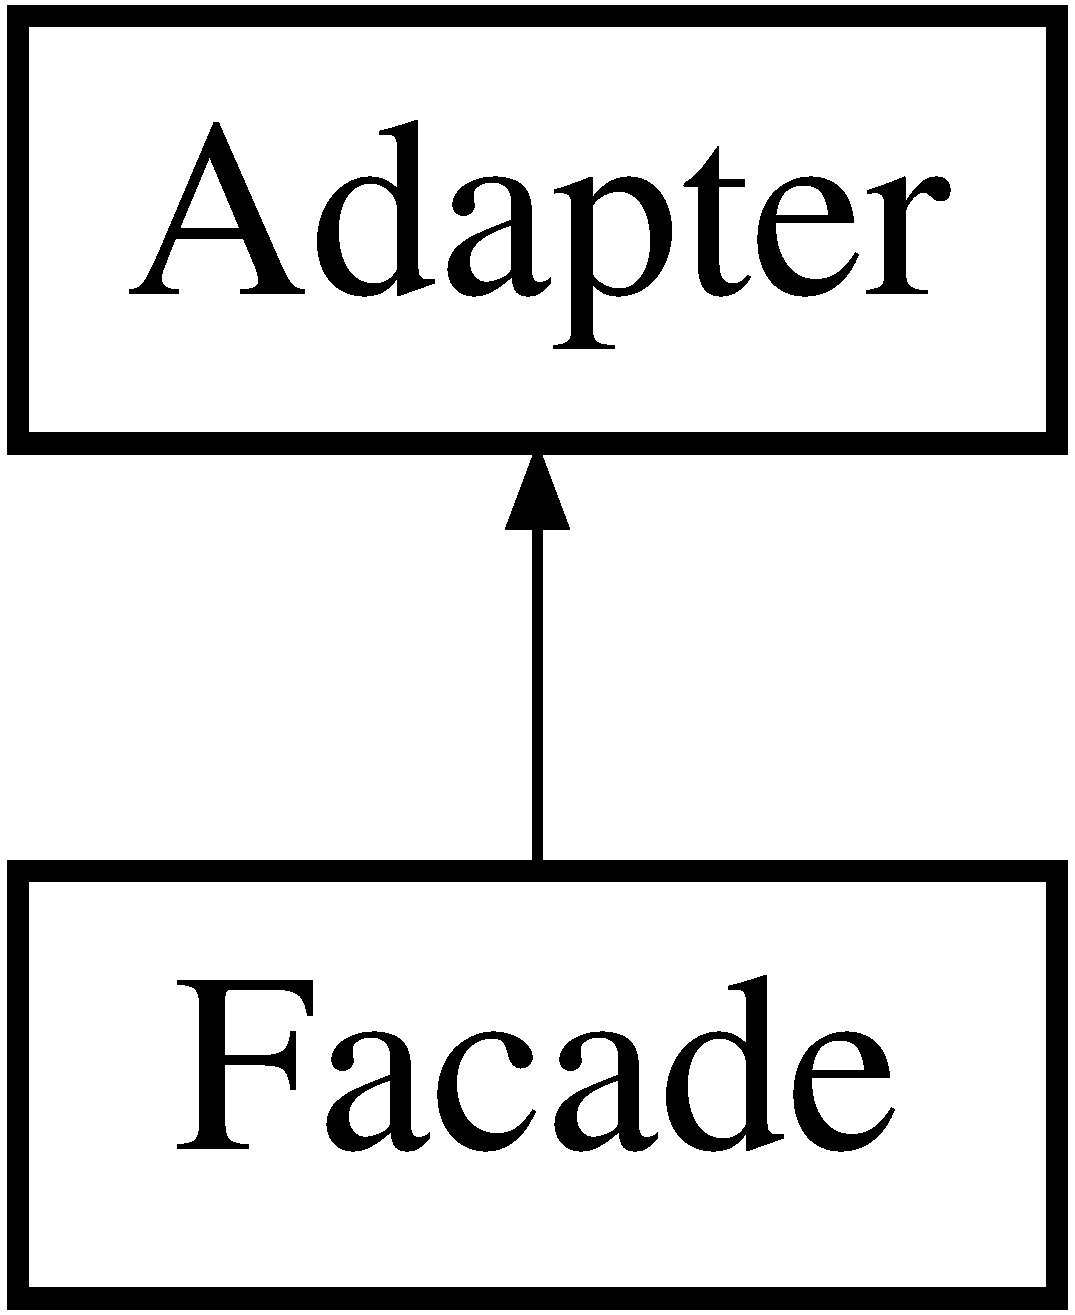
\includegraphics[height=2.000000cm]{classrjakes_1_1_rjakes_simple_f_m_1_1_facade}
\end{center}
\end{figure}
\subsection*{Public Member Functions}
\begin{DoxyCompactItemize}
\item 
\hyperlink{classrjakes_1_1_rjakes_simple_f_m_1_1_facade_a8e9ea0399f612f4a71263951b8d6f058}{set\+Default\+Layout\+Name} (\$fm\+Layout)
\item 
\hyperlink{classrjakes_1_1_rjakes_simple_f_m_1_1_facade_a1467f08efbf646b4487ae46e72489239}{get\+Default\+Layout\+Name} ()
\item 
\hyperlink{classrjakes_1_1_rjakes_simple_f_m_1_1_facade_a4f4ab5b6d37499d3968b93f08e572fc9}{set\+Layout\+Name} (\$fm\+Layout='')
\item 
\hyperlink{classrjakes_1_1_rjakes_simple_f_m_1_1_facade_a2411e5996335b94ed1a325fdedb9dadf}{add\+Where\+Criteria} (\$field, \$value, \$op='')
\item 
\hyperlink{classrjakes_1_1_rjakes_simple_f_m_1_1_facade_ac38bd479da8e3f37484162106d7643e3}{get\+Where\+Criteria} ()
\item 
\hyperlink{classrjakes_1_1_rjakes_simple_f_m_1_1_facade_aae54bb0e269e03e74b14279640de752d}{set\+Where\+Criteria} (\$where\+Criteria)
\item 
\hyperlink{classrjakes_1_1_rjakes_simple_f_m_1_1_facade_add6d4607365ff180fdf20094a5e50217}{add\+Sort\+Criteria} (\$field, \$order='')
\item 
\hyperlink{classrjakes_1_1_rjakes_simple_f_m_1_1_facade_a2e8f539709d5df677aa7827d89812a13}{set\+Sort\+Criteria} (\$sort\+Criteria)
\item 
\hyperlink{classrjakes_1_1_rjakes_simple_f_m_1_1_facade_a7461a494a7f33e439de0faccc6ff1b69}{get\+Sort\+Criteria} ()
\item 
\hyperlink{classrjakes_1_1_rjakes_simple_f_m_1_1_facade_a897a2e727662afedbe8ba63be9b23f1e}{delete} (\$rec\+Id, \$fm\+Layout='')
\item 
\hyperlink{classrjakes_1_1_rjakes_simple_f_m_1_1_facade_a7d04dbb9678b35646853cd186bfc6ed3}{duplicate} (\$rec\+Id, \$fm\+Layout='')
\item 
\hyperlink{classrjakes_1_1_rjakes_simple_f_m_1_1_facade_a20d42898dc5e473f6ac64b2373630ef4}{update} (\$rec\+Id, \$value\+Array, \$fm\+Layout='')
\item 
\hyperlink{classrjakes_1_1_rjakes_simple_f_m_1_1_facade_adba41108fef3c0f2f695f3852b1411d5}{select} (\$max='', \$skip='', \$fm\+Layout='')
\item 
\hyperlink{classrjakes_1_1_rjakes_simple_f_m_1_1_facade_af94c0a2c011aed68ee16e4d5d1bacd57}{insert} (\$value\+Array, \$fm\+Layout='')
\item 
\hyperlink{classrjakes_1_1_rjakes_simple_f_m_1_1_facade_af45812e24c97634b10726423d9571bb5}{set\+Script\+Name} (\$script\+Name)
\item 
\hyperlink{classrjakes_1_1_rjakes_simple_f_m_1_1_facade_a8fddbb7824b34991274f7a3e1211f556}{get\+Script\+Name} ()
\item 
\hyperlink{classrjakes_1_1_rjakes_simple_f_m_1_1_facade_adf0e446c1766376d4e96b4c1e88ef092}{add\+Script\+Parameter} (\$name, \$value)
\item 
\hyperlink{classrjakes_1_1_rjakes_simple_f_m_1_1_facade_a46f7aea523e355126fcbdf6d73832341}{set\+Script\+Parameters} (\$script\+Parameters)
\item 
\hyperlink{classrjakes_1_1_rjakes_simple_f_m_1_1_facade_aaa54c2015868fd4268d2c67afffbbd23}{get\+Script\+Parameters} ()
\item 
\hyperlink{classrjakes_1_1_rjakes_simple_f_m_1_1_facade_aca005e47f884207d90f84fb9461dc5bb}{make\+Script\+Command} ()
\item 
\hyperlink{classrjakes_1_1_rjakes_simple_f_m_1_1_facade_a641a0b194ef0f1f5ec42ef7f41bb4447}{execute\+Fm\+Script} (\$script= '', \$fm\+Layout='')
\end{DoxyCompactItemize}
\subsection*{Protected Attributes}
\begin{DoxyCompactItemize}
\item 
\hypertarget{classrjakes_1_1_rjakes_simple_f_m_1_1_facade_acee9fef38dab29dc51d335ce0d3bb12f}{{\bfseries \$default\+Layout\+Name} = ''}\label{classrjakes_1_1_rjakes_simple_f_m_1_1_facade_acee9fef38dab29dc51d335ce0d3bb12f}

\item 
\hypertarget{classrjakes_1_1_rjakes_simple_f_m_1_1_facade_ac80a8ebff266cd68c5d4f5735335109f}{{\bfseries \$where\+Criteria} = array()}\label{classrjakes_1_1_rjakes_simple_f_m_1_1_facade_ac80a8ebff266cd68c5d4f5735335109f}

\item 
\hypertarget{classrjakes_1_1_rjakes_simple_f_m_1_1_facade_a5d7448ed2dd9d65e98b922cc4c686234}{{\bfseries \$sort\+Criteria} = array()}\label{classrjakes_1_1_rjakes_simple_f_m_1_1_facade_a5d7448ed2dd9d65e98b922cc4c686234}

\item 
\hypertarget{classrjakes_1_1_rjakes_simple_f_m_1_1_facade_a7dccab22d88281f5f621207815521b79}{{\bfseries \$script\+Name} = ''}\label{classrjakes_1_1_rjakes_simple_f_m_1_1_facade_a7dccab22d88281f5f621207815521b79}

\item 
\hypertarget{classrjakes_1_1_rjakes_simple_f_m_1_1_facade_ac9f0bb23ade1512d0f500c4fc55a4dda}{{\bfseries \$script\+Parameters} = array()}\label{classrjakes_1_1_rjakes_simple_f_m_1_1_facade_ac9f0bb23ade1512d0f500c4fc55a4dda}

\end{DoxyCompactItemize}


\subsection{Member Function Documentation}
\hypertarget{classrjakes_1_1_rjakes_simple_f_m_1_1_facade_adf0e446c1766376d4e96b4c1e88ef092}{\index{rjakes\+::\+Rjakes\+Simple\+F\+M\+::\+Facade@{rjakes\+::\+Rjakes\+Simple\+F\+M\+::\+Facade}!add\+Script\+Parameter@{add\+Script\+Parameter}}
\index{add\+Script\+Parameter@{add\+Script\+Parameter}!rjakes\+::\+Rjakes\+Simple\+F\+M\+::\+Facade@{rjakes\+::\+Rjakes\+Simple\+F\+M\+::\+Facade}}
\subsubsection[{add\+Script\+Parameter}]{\setlength{\rightskip}{0pt plus 5cm}add\+Script\+Parameter (
\begin{DoxyParamCaption}
\item[{}]{\$name, }
\item[{}]{\$value}
\end{DoxyParamCaption}
)}}\label{classrjakes_1_1_rjakes_simple_f_m_1_1_facade_adf0e446c1766376d4e96b4c1e88ef092}
Add a single named script parameter to be sent to the File\+Maker script 
\begin{DoxyParams}[1]{Parameters}
string & {\em \$name} & \\
\hline
string & {\em \$value} & \\
\hline
\end{DoxyParams}
\begin{DoxyReturn}{Returns}
object of class \hyperlink{classrjakes_1_1_rjakes_simple_f_m_1_1_facade}{Rjakes\+Simple\+F\+M\+::\+Facade} 
\end{DoxyReturn}
\hypertarget{classrjakes_1_1_rjakes_simple_f_m_1_1_facade_add6d4607365ff180fdf20094a5e50217}{\index{rjakes\+::\+Rjakes\+Simple\+F\+M\+::\+Facade@{rjakes\+::\+Rjakes\+Simple\+F\+M\+::\+Facade}!add\+Sort\+Criteria@{add\+Sort\+Criteria}}
\index{add\+Sort\+Criteria@{add\+Sort\+Criteria}!rjakes\+::\+Rjakes\+Simple\+F\+M\+::\+Facade@{rjakes\+::\+Rjakes\+Simple\+F\+M\+::\+Facade}}
\subsubsection[{add\+Sort\+Criteria}]{\setlength{\rightskip}{0pt plus 5cm}add\+Sort\+Criteria (
\begin{DoxyParamCaption}
\item[{}]{\$field, }
\item[{}]{\$order = {\ttfamily ''}}
\end{DoxyParamCaption}
)}}\label{classrjakes_1_1_rjakes_simple_f_m_1_1_facade_add6d4607365ff180fdf20094a5e50217}
Add a single set of sort criteria to the sort criteria array property. 
\begin{DoxyParams}[1]{Parameters}
string & {\em \$field} & \\
\hline
string & {\em \$order} & order is 'ascend' or 'descend' \\
\hline
\end{DoxyParams}
\begin{DoxyReturn}{Returns}
object of class \hyperlink{classrjakes_1_1_rjakes_simple_f_m_1_1_facade}{Rjakes\+Simple\+F\+M\+::\+Facade} 
\end{DoxyReturn}
\hypertarget{classrjakes_1_1_rjakes_simple_f_m_1_1_facade_a2411e5996335b94ed1a325fdedb9dadf}{\index{rjakes\+::\+Rjakes\+Simple\+F\+M\+::\+Facade@{rjakes\+::\+Rjakes\+Simple\+F\+M\+::\+Facade}!add\+Where\+Criteria@{add\+Where\+Criteria}}
\index{add\+Where\+Criteria@{add\+Where\+Criteria}!rjakes\+::\+Rjakes\+Simple\+F\+M\+::\+Facade@{rjakes\+::\+Rjakes\+Simple\+F\+M\+::\+Facade}}
\subsubsection[{add\+Where\+Criteria}]{\setlength{\rightskip}{0pt plus 5cm}add\+Where\+Criteria (
\begin{DoxyParamCaption}
\item[{}]{\$field, }
\item[{}]{\$value, }
\item[{}]{\$op = {\ttfamily ''}}
\end{DoxyParamCaption}
)}}\label{classrjakes_1_1_rjakes_simple_f_m_1_1_facade_a2411e5996335b94ed1a325fdedb9dadf}
Add a single where/find criteria. 
\begin{DoxyParams}[1]{Parameters}
string & {\em \$field} & \\
\hline
string & {\em \$value} & \\
\hline
string & {\em \$op} & 
\begin{DoxyItemize}
\item Operators\+:
\item eq (equals)
\item cn (contains)
\item bw (begins with)
\item ew (ends with)
\item gt (greater than)
\item gte (greater than or equal to)
\item lt (less than)
\item lte (less than or equal to)
\item neq (not equal) 
\end{DoxyItemize}\\
\hline
\end{DoxyParams}
\begin{DoxyReturn}{Returns}
object of class \hyperlink{classrjakes_1_1_rjakes_simple_f_m_1_1_facade}{Rjakes\+Simple\+F\+M\+::\+Facade} 
\end{DoxyReturn}
\hypertarget{classrjakes_1_1_rjakes_simple_f_m_1_1_facade_a897a2e727662afedbe8ba63be9b23f1e}{\index{rjakes\+::\+Rjakes\+Simple\+F\+M\+::\+Facade@{rjakes\+::\+Rjakes\+Simple\+F\+M\+::\+Facade}!delete@{delete}}
\index{delete@{delete}!rjakes\+::\+Rjakes\+Simple\+F\+M\+::\+Facade@{rjakes\+::\+Rjakes\+Simple\+F\+M\+::\+Facade}}
\subsubsection[{delete}]{\setlength{\rightskip}{0pt plus 5cm}delete (
\begin{DoxyParamCaption}
\item[{}]{\$rec\+Id, }
\item[{}]{\$fm\+Layout = {\ttfamily ''}}
\end{DoxyParamCaption}
)}}\label{classrjakes_1_1_rjakes_simple_f_m_1_1_facade_a897a2e727662afedbe8ba63be9b23f1e}
C\+R\+U\+D function to delete a record. 
\begin{DoxyParams}[1]{Parameters}
string & {\em \$rec\+Id} & This is the internal File\+Maker record\+I\+D. You can get this from C\+R\+U\+D functions that returns database results, within the 'rows' elements \\
\hline
string & {\em \$fm\+Layout} & Optional, if a layout has already been set with \hyperlink{classrjakes_1_1_rjakes_simple_f_m_1_1_facade_a8e9ea0399f612f4a71263951b8d6f058}{set\+Default\+Layout\+Name()} \\
\hline
\end{DoxyParams}
\begin{DoxyReturn}{Returns}
array(\mbox{[}url\mbox{]} \mbox{[}error\mbox{]} \mbox{[}errortext\mbox{]} \mbox{[}errortype\mbox{]} \mbox{[}count\mbox{]} \mbox{[}fetchsize\mbox{]} \mbox{[}rows\mbox{]} =$>$ array) 
\end{DoxyReturn}
\hypertarget{classrjakes_1_1_rjakes_simple_f_m_1_1_facade_a7d04dbb9678b35646853cd186bfc6ed3}{\index{rjakes\+::\+Rjakes\+Simple\+F\+M\+::\+Facade@{rjakes\+::\+Rjakes\+Simple\+F\+M\+::\+Facade}!duplicate@{duplicate}}
\index{duplicate@{duplicate}!rjakes\+::\+Rjakes\+Simple\+F\+M\+::\+Facade@{rjakes\+::\+Rjakes\+Simple\+F\+M\+::\+Facade}}
\subsubsection[{duplicate}]{\setlength{\rightskip}{0pt plus 5cm}duplicate (
\begin{DoxyParamCaption}
\item[{}]{\$rec\+Id, }
\item[{}]{\$fm\+Layout = {\ttfamily ''}}
\end{DoxyParamCaption}
)}}\label{classrjakes_1_1_rjakes_simple_f_m_1_1_facade_a7d04dbb9678b35646853cd186bfc6ed3}
C\+R\+U\+D function to duplicate a record. 
\begin{DoxyParams}[1]{Parameters}
string & {\em \$rec\+Id} & This is the internal File\+Maker record\+I\+D. You can get this from C\+R\+U\+D functions that returns database results, within the 'rows' elements \\
\hline
string & {\em \$fm\+Layout} & Optional, if a layout has already been set with \hyperlink{classrjakes_1_1_rjakes_simple_f_m_1_1_facade_a8e9ea0399f612f4a71263951b8d6f058}{set\+Default\+Layout\+Name()} \\
\hline
\end{DoxyParams}
\begin{DoxyReturn}{Returns}
array(\mbox{[}url\mbox{]} \mbox{[}error\mbox{]} \mbox{[}errortext\mbox{]} \mbox{[}errortype\mbox{]} \mbox{[}count\mbox{]} \mbox{[}fetchsize\mbox{]} \mbox{[}rows\mbox{]} =$>$ array) 
\end{DoxyReturn}
\hypertarget{classrjakes_1_1_rjakes_simple_f_m_1_1_facade_a641a0b194ef0f1f5ec42ef7f41bb4447}{\index{rjakes\+::\+Rjakes\+Simple\+F\+M\+::\+Facade@{rjakes\+::\+Rjakes\+Simple\+F\+M\+::\+Facade}!execute\+Fm\+Script@{execute\+Fm\+Script}}
\index{execute\+Fm\+Script@{execute\+Fm\+Script}!rjakes\+::\+Rjakes\+Simple\+F\+M\+::\+Facade@{rjakes\+::\+Rjakes\+Simple\+F\+M\+::\+Facade}}
\subsubsection[{execute\+Fm\+Script}]{\setlength{\rightskip}{0pt plus 5cm}execute\+Fm\+Script (
\begin{DoxyParamCaption}
\item[{}]{\$script = {\ttfamily ''}, }
\item[{}]{\$fm\+Layout = {\ttfamily ''}}
\end{DoxyParamCaption}
)}}\label{classrjakes_1_1_rjakes_simple_f_m_1_1_facade_a641a0b194ef0f1f5ec42ef7f41bb4447}
Executes a File\+Maker script independent of a C\+R\+U\+D request, using the \$script\+Name property and any parameters in \$script\+Parameters 
\begin{DoxyParams}[1]{Parameters}
string & {\em \$script} & Optional if \$script\+Name property is set. \\
\hline
string & {\em \$fm\+Layout} & Optional if \$default\+Layout\+Name is set. \\
\hline
\end{DoxyParams}
\begin{DoxyReturn}{Returns}
array(\mbox{[}url\mbox{]} \mbox{[}error\mbox{]} \mbox{[}errortext\mbox{]} \mbox{[}errortype\mbox{]} \mbox{[}count\mbox{]} \mbox{[}fetchsize\mbox{]} \mbox{[}rows\mbox{]} =$>$ array) 
\end{DoxyReturn}
\begin{DoxyRefDesc}{Todo}
\item[\hyperlink{todo__todo000001}{Todo}]Throw as exception for missing layout\+Name or script\+Name \end{DoxyRefDesc}
\hypertarget{classrjakes_1_1_rjakes_simple_f_m_1_1_facade_a1467f08efbf646b4487ae46e72489239}{\index{rjakes\+::\+Rjakes\+Simple\+F\+M\+::\+Facade@{rjakes\+::\+Rjakes\+Simple\+F\+M\+::\+Facade}!get\+Default\+Layout\+Name@{get\+Default\+Layout\+Name}}
\index{get\+Default\+Layout\+Name@{get\+Default\+Layout\+Name}!rjakes\+::\+Rjakes\+Simple\+F\+M\+::\+Facade@{rjakes\+::\+Rjakes\+Simple\+F\+M\+::\+Facade}}
\subsubsection[{get\+Default\+Layout\+Name}]{\setlength{\rightskip}{0pt plus 5cm}get\+Default\+Layout\+Name (
\begin{DoxyParamCaption}
{}
\end{DoxyParamCaption}
)}}\label{classrjakes_1_1_rjakes_simple_f_m_1_1_facade_a1467f08efbf646b4487ae46e72489239}
Get the default File\+Maker layout name. \begin{DoxyReturn}{Returns}
string 
\end{DoxyReturn}
\hypertarget{classrjakes_1_1_rjakes_simple_f_m_1_1_facade_a8fddbb7824b34991274f7a3e1211f556}{\index{rjakes\+::\+Rjakes\+Simple\+F\+M\+::\+Facade@{rjakes\+::\+Rjakes\+Simple\+F\+M\+::\+Facade}!get\+Script\+Name@{get\+Script\+Name}}
\index{get\+Script\+Name@{get\+Script\+Name}!rjakes\+::\+Rjakes\+Simple\+F\+M\+::\+Facade@{rjakes\+::\+Rjakes\+Simple\+F\+M\+::\+Facade}}
\subsubsection[{get\+Script\+Name}]{\setlength{\rightskip}{0pt plus 5cm}get\+Script\+Name (
\begin{DoxyParamCaption}
{}
\end{DoxyParamCaption}
)}}\label{classrjakes_1_1_rjakes_simple_f_m_1_1_facade_a8fddbb7824b34991274f7a3e1211f556}
Get the \$script\+Name property, if populated \begin{DoxyReturn}{Returns}
string 
\end{DoxyReturn}
\hypertarget{classrjakes_1_1_rjakes_simple_f_m_1_1_facade_aaa54c2015868fd4268d2c67afffbbd23}{\index{rjakes\+::\+Rjakes\+Simple\+F\+M\+::\+Facade@{rjakes\+::\+Rjakes\+Simple\+F\+M\+::\+Facade}!get\+Script\+Parameters@{get\+Script\+Parameters}}
\index{get\+Script\+Parameters@{get\+Script\+Parameters}!rjakes\+::\+Rjakes\+Simple\+F\+M\+::\+Facade@{rjakes\+::\+Rjakes\+Simple\+F\+M\+::\+Facade}}
\subsubsection[{get\+Script\+Parameters}]{\setlength{\rightskip}{0pt plus 5cm}get\+Script\+Parameters (
\begin{DoxyParamCaption}
{}
\end{DoxyParamCaption}
)}}\label{classrjakes_1_1_rjakes_simple_f_m_1_1_facade_aaa54c2015868fd4268d2c67afffbbd23}
Get the multi dimensional \$script\+Parameters property \begin{DoxyReturn}{Returns}
array ( array(\mbox{[}name\mbox{]}=$>$'some\+Parm\+Name', \mbox{[}value\mbox{]}=$>$'some parm value')) 
\end{DoxyReturn}
\hypertarget{classrjakes_1_1_rjakes_simple_f_m_1_1_facade_a7461a494a7f33e439de0faccc6ff1b69}{\index{rjakes\+::\+Rjakes\+Simple\+F\+M\+::\+Facade@{rjakes\+::\+Rjakes\+Simple\+F\+M\+::\+Facade}!get\+Sort\+Criteria@{get\+Sort\+Criteria}}
\index{get\+Sort\+Criteria@{get\+Sort\+Criteria}!rjakes\+::\+Rjakes\+Simple\+F\+M\+::\+Facade@{rjakes\+::\+Rjakes\+Simple\+F\+M\+::\+Facade}}
\subsubsection[{get\+Sort\+Criteria}]{\setlength{\rightskip}{0pt plus 5cm}get\+Sort\+Criteria (
\begin{DoxyParamCaption}
{}
\end{DoxyParamCaption}
)}}\label{classrjakes_1_1_rjakes_simple_f_m_1_1_facade_a7461a494a7f33e439de0faccc6ff1b69}
Get the multi dimensional array of \$sort\+Criteria property. \begin{DoxyReturn}{Returns}
array( array(\$field, \$order) ) 
\end{DoxyReturn}
\hypertarget{classrjakes_1_1_rjakes_simple_f_m_1_1_facade_ac38bd479da8e3f37484162106d7643e3}{\index{rjakes\+::\+Rjakes\+Simple\+F\+M\+::\+Facade@{rjakes\+::\+Rjakes\+Simple\+F\+M\+::\+Facade}!get\+Where\+Criteria@{get\+Where\+Criteria}}
\index{get\+Where\+Criteria@{get\+Where\+Criteria}!rjakes\+::\+Rjakes\+Simple\+F\+M\+::\+Facade@{rjakes\+::\+Rjakes\+Simple\+F\+M\+::\+Facade}}
\subsubsection[{get\+Where\+Criteria}]{\setlength{\rightskip}{0pt plus 5cm}get\+Where\+Criteria (
\begin{DoxyParamCaption}
{}
\end{DoxyParamCaption}
)}}\label{classrjakes_1_1_rjakes_simple_f_m_1_1_facade_ac38bd479da8e3f37484162106d7643e3}
Return the multi dimensional array of sort criteria \begin{DoxyReturn}{Returns}
array ( array(\$field, \$value, \$operator)) 
\end{DoxyReturn}
\hypertarget{classrjakes_1_1_rjakes_simple_f_m_1_1_facade_af94c0a2c011aed68ee16e4d5d1bacd57}{\index{rjakes\+::\+Rjakes\+Simple\+F\+M\+::\+Facade@{rjakes\+::\+Rjakes\+Simple\+F\+M\+::\+Facade}!insert@{insert}}
\index{insert@{insert}!rjakes\+::\+Rjakes\+Simple\+F\+M\+::\+Facade@{rjakes\+::\+Rjakes\+Simple\+F\+M\+::\+Facade}}
\subsubsection[{insert}]{\setlength{\rightskip}{0pt plus 5cm}insert (
\begin{DoxyParamCaption}
\item[{}]{\$value\+Array, }
\item[{}]{\$fm\+Layout = {\ttfamily ''}}
\end{DoxyParamCaption}
)}}\label{classrjakes_1_1_rjakes_simple_f_m_1_1_facade_af94c0a2c011aed68ee16e4d5d1bacd57}
C\+R\+U\+D function to insert a record. 
\begin{DoxyParams}[1]{Parameters}
array & {\em \$value\+Array} & = array('field\+Name' =$>$ 'value', 'another\+Field\+Name' =$>$ 'value') \\
\hline
string & {\em \$fm\+Layout} & Optional, if a layout has already been set with \hyperlink{classrjakes_1_1_rjakes_simple_f_m_1_1_facade_a8e9ea0399f612f4a71263951b8d6f058}{set\+Default\+Layout\+Name()} \\
\hline
\end{DoxyParams}
\begin{DoxyReturn}{Returns}
array(\mbox{[}url\mbox{]} \mbox{[}error\mbox{]} \mbox{[}errortext\mbox{]} \mbox{[}errortype\mbox{]} \mbox{[}count\mbox{]} \mbox{[}fetchsize\mbox{]} \mbox{[}rows\mbox{]} =$>$ array) 
\end{DoxyReturn}
\hypertarget{classrjakes_1_1_rjakes_simple_f_m_1_1_facade_aca005e47f884207d90f84fb9461dc5bb}{\index{rjakes\+::\+Rjakes\+Simple\+F\+M\+::\+Facade@{rjakes\+::\+Rjakes\+Simple\+F\+M\+::\+Facade}!make\+Script\+Command@{make\+Script\+Command}}
\index{make\+Script\+Command@{make\+Script\+Command}!rjakes\+::\+Rjakes\+Simple\+F\+M\+::\+Facade@{rjakes\+::\+Rjakes\+Simple\+F\+M\+::\+Facade}}
\subsubsection[{make\+Script\+Command}]{\setlength{\rightskip}{0pt plus 5cm}make\+Script\+Command (
\begin{DoxyParamCaption}
{}
\end{DoxyParamCaption}
)}}\label{classrjakes_1_1_rjakes_simple_f_m_1_1_facade_aca005e47f884207d90f84fb9461dc5bb}
Makes the name value pairs needed to execute a File\+Maker script from an http request \begin{DoxyReturn}{Returns}
string 
\end{DoxyReturn}
\hypertarget{classrjakes_1_1_rjakes_simple_f_m_1_1_facade_adba41108fef3c0f2f695f3852b1411d5}{\index{rjakes\+::\+Rjakes\+Simple\+F\+M\+::\+Facade@{rjakes\+::\+Rjakes\+Simple\+F\+M\+::\+Facade}!select@{select}}
\index{select@{select}!rjakes\+::\+Rjakes\+Simple\+F\+M\+::\+Facade@{rjakes\+::\+Rjakes\+Simple\+F\+M\+::\+Facade}}
\subsubsection[{select}]{\setlength{\rightskip}{0pt plus 5cm}select (
\begin{DoxyParamCaption}
\item[{}]{\$max = {\ttfamily ''}, }
\item[{}]{\$skip = {\ttfamily ''}, }
\item[{}]{\$fm\+Layout = {\ttfamily ''}}
\end{DoxyParamCaption}
)}}\label{classrjakes_1_1_rjakes_simple_f_m_1_1_facade_adba41108fef3c0f2f695f3852b1411d5}
C\+R\+U\+D function to retrieve records. The properties of \$sort\+Criteria, \$where\+Criteria,and \$script\+Name are used, if populated. 
\begin{DoxyParams}[1]{Parameters}
string & {\em \$max} & \\
\hline
string & {\em \$skip} & \\
\hline
string & {\em \$fm\+Layout} & Optional, if a layout has already been set with \hyperlink{classrjakes_1_1_rjakes_simple_f_m_1_1_facade_a8e9ea0399f612f4a71263951b8d6f058}{set\+Default\+Layout\+Name()} \\
\hline
\end{DoxyParams}
\begin{DoxyReturn}{Returns}
array(\mbox{[}url\mbox{]} \mbox{[}error\mbox{]} \mbox{[}errortext\mbox{]} \mbox{[}errortype\mbox{]} \mbox{[}count\mbox{]} \mbox{[}fetchsize\mbox{]} \mbox{[}rows\mbox{]} =$>$ array) 
\end{DoxyReturn}
\hypertarget{classrjakes_1_1_rjakes_simple_f_m_1_1_facade_a8e9ea0399f612f4a71263951b8d6f058}{\index{rjakes\+::\+Rjakes\+Simple\+F\+M\+::\+Facade@{rjakes\+::\+Rjakes\+Simple\+F\+M\+::\+Facade}!set\+Default\+Layout\+Name@{set\+Default\+Layout\+Name}}
\index{set\+Default\+Layout\+Name@{set\+Default\+Layout\+Name}!rjakes\+::\+Rjakes\+Simple\+F\+M\+::\+Facade@{rjakes\+::\+Rjakes\+Simple\+F\+M\+::\+Facade}}
\subsubsection[{set\+Default\+Layout\+Name}]{\setlength{\rightskip}{0pt plus 5cm}set\+Default\+Layout\+Name (
\begin{DoxyParamCaption}
\item[{}]{\$fm\+Layout}
\end{DoxyParamCaption}
)}}\label{classrjakes_1_1_rjakes_simple_f_m_1_1_facade_a8e9ea0399f612f4a71263951b8d6f058}
Set a default layout name, so that C\+R\+U\+D functions can be called without a layout name. 
\begin{DoxyParams}[1]{Parameters}
string & {\em \$fm\+Layout} & \\
\hline
\end{DoxyParams}
\begin{DoxyReturn}{Returns}
object of class \hyperlink{classrjakes_1_1_rjakes_simple_f_m_1_1_facade}{Rjakes\+Simple\+F\+M\+::\+Facade} 
\end{DoxyReturn}
\hypertarget{classrjakes_1_1_rjakes_simple_f_m_1_1_facade_a4f4ab5b6d37499d3968b93f08e572fc9}{\index{rjakes\+::\+Rjakes\+Simple\+F\+M\+::\+Facade@{rjakes\+::\+Rjakes\+Simple\+F\+M\+::\+Facade}!set\+Layout\+Name@{set\+Layout\+Name}}
\index{set\+Layout\+Name@{set\+Layout\+Name}!rjakes\+::\+Rjakes\+Simple\+F\+M\+::\+Facade@{rjakes\+::\+Rjakes\+Simple\+F\+M\+::\+Facade}}
\subsubsection[{set\+Layout\+Name}]{\setlength{\rightskip}{0pt plus 5cm}set\+Layout\+Name (
\begin{DoxyParamCaption}
\item[{}]{\$fm\+Layout = {\ttfamily ''}}
\end{DoxyParamCaption}
)}}\label{classrjakes_1_1_rjakes_simple_f_m_1_1_facade_a4f4ab5b6d37499d3968b93f08e572fc9}
Overrides Simple\+F\+M so that we can use a default layout. 
\begin{DoxyParams}[1]{Parameters}
string & {\em \$fm\+Layout} & \\
\hline
\end{DoxyParams}
\begin{DoxyReturn}{Returns}
object of class \hyperlink{classrjakes_1_1_rjakes_simple_f_m_1_1_facade}{Rjakes\+Simple\+F\+M\+::\+Facade} 
\end{DoxyReturn}
\hypertarget{classrjakes_1_1_rjakes_simple_f_m_1_1_facade_af45812e24c97634b10726423d9571bb5}{\index{rjakes\+::\+Rjakes\+Simple\+F\+M\+::\+Facade@{rjakes\+::\+Rjakes\+Simple\+F\+M\+::\+Facade}!set\+Script\+Name@{set\+Script\+Name}}
\index{set\+Script\+Name@{set\+Script\+Name}!rjakes\+::\+Rjakes\+Simple\+F\+M\+::\+Facade@{rjakes\+::\+Rjakes\+Simple\+F\+M\+::\+Facade}}
\subsubsection[{set\+Script\+Name}]{\setlength{\rightskip}{0pt plus 5cm}set\+Script\+Name (
\begin{DoxyParamCaption}
\item[{}]{\$script\+Name}
\end{DoxyParamCaption}
)}}\label{classrjakes_1_1_rjakes_simple_f_m_1_1_facade_af45812e24c97634b10726423d9571bb5}
Overwrite the \$script\+Name property with a File\+Maker script name 
\begin{DoxyParams}[1]{Parameters}
string & {\em \$script\+Name} & \\
\hline
\end{DoxyParams}
\begin{DoxyReturn}{Returns}
object of class \hyperlink{classrjakes_1_1_rjakes_simple_f_m_1_1_facade}{Rjakes\+Simple\+F\+M\+::\+Facade} 
\end{DoxyReturn}
\hypertarget{classrjakes_1_1_rjakes_simple_f_m_1_1_facade_a46f7aea523e355126fcbdf6d73832341}{\index{rjakes\+::\+Rjakes\+Simple\+F\+M\+::\+Facade@{rjakes\+::\+Rjakes\+Simple\+F\+M\+::\+Facade}!set\+Script\+Parameters@{set\+Script\+Parameters}}
\index{set\+Script\+Parameters@{set\+Script\+Parameters}!rjakes\+::\+Rjakes\+Simple\+F\+M\+::\+Facade@{rjakes\+::\+Rjakes\+Simple\+F\+M\+::\+Facade}}
\subsubsection[{set\+Script\+Parameters}]{\setlength{\rightskip}{0pt plus 5cm}set\+Script\+Parameters (
\begin{DoxyParamCaption}
\item[{}]{\$script\+Parameters}
\end{DoxyParamCaption}
)}}\label{classrjakes_1_1_rjakes_simple_f_m_1_1_facade_a46f7aea523e355126fcbdf6d73832341}
Overwrite the \$script\+Parameters multi dimensional array property with an array of script parameter arrays 
\begin{DoxyParams}[1]{Parameters}
array & {\em \$script\+Parameters} & array ( array(\mbox{[}name\mbox{]}=$>$'some\+Parm\+Name', \mbox{[}value\mbox{]}=$>$'some parm value')) \\
\hline
\end{DoxyParams}
\begin{DoxyReturn}{Returns}
object of class \hyperlink{classrjakes_1_1_rjakes_simple_f_m_1_1_facade}{Rjakes\+Simple\+F\+M\+::\+Facade} 
\end{DoxyReturn}
\hypertarget{classrjakes_1_1_rjakes_simple_f_m_1_1_facade_a2e8f539709d5df677aa7827d89812a13}{\index{rjakes\+::\+Rjakes\+Simple\+F\+M\+::\+Facade@{rjakes\+::\+Rjakes\+Simple\+F\+M\+::\+Facade}!set\+Sort\+Criteria@{set\+Sort\+Criteria}}
\index{set\+Sort\+Criteria@{set\+Sort\+Criteria}!rjakes\+::\+Rjakes\+Simple\+F\+M\+::\+Facade@{rjakes\+::\+Rjakes\+Simple\+F\+M\+::\+Facade}}
\subsubsection[{set\+Sort\+Criteria}]{\setlength{\rightskip}{0pt plus 5cm}set\+Sort\+Criteria (
\begin{DoxyParamCaption}
\item[{}]{\$sort\+Criteria}
\end{DoxyParamCaption}
)}}\label{classrjakes_1_1_rjakes_simple_f_m_1_1_facade_a2e8f539709d5df677aa7827d89812a13}
Overwrite the \$sort\+Criteria array property with an array of sort criteria arrays. 
\begin{DoxyParams}[1]{Parameters}
array & {\em \$sort\+Criteria} & array( array(\$field, \$order) ) order is 'ascend' or 'descend'. \\
\hline
\end{DoxyParams}
\begin{DoxyReturn}{Returns}
object of class \hyperlink{classrjakes_1_1_rjakes_simple_f_m_1_1_facade}{Rjakes\+Simple\+F\+M\+::\+Facade} 
\end{DoxyReturn}
\hypertarget{classrjakes_1_1_rjakes_simple_f_m_1_1_facade_aae54bb0e269e03e74b14279640de752d}{\index{rjakes\+::\+Rjakes\+Simple\+F\+M\+::\+Facade@{rjakes\+::\+Rjakes\+Simple\+F\+M\+::\+Facade}!set\+Where\+Criteria@{set\+Where\+Criteria}}
\index{set\+Where\+Criteria@{set\+Where\+Criteria}!rjakes\+::\+Rjakes\+Simple\+F\+M\+::\+Facade@{rjakes\+::\+Rjakes\+Simple\+F\+M\+::\+Facade}}
\subsubsection[{set\+Where\+Criteria}]{\setlength{\rightskip}{0pt plus 5cm}set\+Where\+Criteria (
\begin{DoxyParamCaption}
\item[{}]{\$where\+Criteria}
\end{DoxyParamCaption}
)}}\label{classrjakes_1_1_rjakes_simple_f_m_1_1_facade_aae54bb0e269e03e74b14279640de752d}
Overwrite the where criteria array property with an array of where criteria arrays. 
\begin{DoxyParams}[1]{Parameters}
array & {\em \$where\+Criteria} & array( array('field' =$>$ 'some\+Field\+Name', 'value' =$>$ 'some value', 'op' =$>$ 'an operator')).
\begin{DoxyItemize}
\item Operators\+:
\item eq (equals)
\item cn (contains)
\item bw (begins with)
\item ew (ends with)
\item gt (greater than)
\item gte (greater than or equal to)
\item lt (less than)
\item lte (less than or equal to)
\item neq (not equal) 
\end{DoxyItemize}\\
\hline
\end{DoxyParams}
\begin{DoxyReturn}{Returns}
object of class \hyperlink{classrjakes_1_1_rjakes_simple_f_m_1_1_facade}{Rjakes\+Simple\+F\+M\+::\+Facade}. 
\end{DoxyReturn}
\hypertarget{classrjakes_1_1_rjakes_simple_f_m_1_1_facade_a20d42898dc5e473f6ac64b2373630ef4}{\index{rjakes\+::\+Rjakes\+Simple\+F\+M\+::\+Facade@{rjakes\+::\+Rjakes\+Simple\+F\+M\+::\+Facade}!update@{update}}
\index{update@{update}!rjakes\+::\+Rjakes\+Simple\+F\+M\+::\+Facade@{rjakes\+::\+Rjakes\+Simple\+F\+M\+::\+Facade}}
\subsubsection[{update}]{\setlength{\rightskip}{0pt plus 5cm}update (
\begin{DoxyParamCaption}
\item[{}]{\$rec\+Id, }
\item[{}]{\$value\+Array, }
\item[{}]{\$fm\+Layout = {\ttfamily ''}}
\end{DoxyParamCaption}
)}}\label{classrjakes_1_1_rjakes_simple_f_m_1_1_facade_a20d42898dc5e473f6ac64b2373630ef4}
C\+R\+U\+D function to update a record. 
\begin{DoxyParams}[1]{Parameters}
string & {\em \$rec\+Id} & This is the internal File\+Maker record\+I\+D. You can get this from C\+R\+U\+D function that returns database results, within the 'rows' elements \\
\hline
array & {\em \$value\+Array} & array('field\+Name' =$>$ 'value', 'another\+Field\+Name' =$>$ 'value') \\
\hline
string & {\em \$fm\+Layout} & Optional, if a layout has already been set with \hyperlink{classrjakes_1_1_rjakes_simple_f_m_1_1_facade_a8e9ea0399f612f4a71263951b8d6f058}{set\+Default\+Layout\+Name()} \\
\hline
\end{DoxyParams}
\begin{DoxyReturn}{Returns}
array(\mbox{[}url\mbox{]} \mbox{[}error\mbox{]} \mbox{[}errortext\mbox{]} \mbox{[}errortype\mbox{]} \mbox{[}count\mbox{]} \mbox{[}fetchsize\mbox{]} \mbox{[}rows\mbox{]} =$>$ array) 
\end{DoxyReturn}


The documentation for this class was generated from the following file\+:\begin{DoxyCompactItemize}
\item 
/\+Library/\+Web\+Server/\+Documents/vhosts/uic\+\_\+sites/fuel/vendor/rjakes/rjakessimplefm/library/rjakes/\+Rjakes\+Simple\+F\+M/Facade.\+php\end{DoxyCompactItemize}

\hypertarget{classrjakes_1_1_rjakes_simple_f_m_1_1_version}{\section{Version Class Reference}
\label{classrjakes_1_1_rjakes_simple_f_m_1_1_version}\index{Version@{Version}}
}
\subsection*{Data Fields}
\begin{DoxyCompactItemize}
\item 
\hypertarget{classrjakes_1_1_rjakes_simple_f_m_1_1_version_af71005841ce53adac00581ab0ba24c1f}{const {\bfseries V\+E\+R\+S\+I\+O\+N} = '0.\+0.\+0alpha2'}\label{classrjakes_1_1_rjakes_simple_f_m_1_1_version_af71005841ce53adac00581ab0ba24c1f}

\end{DoxyCompactItemize}


The documentation for this class was generated from the following file\+:\begin{DoxyCompactItemize}
\item 
/\+Library/\+Web\+Server/\+Documents/vhosts/uic\+\_\+sites/fuel/vendor/rjakes/rjakessimplefm/library/rjakes/\+Rjakes\+Simple\+F\+M/Version.\+php\end{DoxyCompactItemize}

%--- End generated contents ---

% Index
\newpage
\phantomsection
\addcontentsline{toc}{chapter}{Index}
\printindex

\end{document}
